\documentclass{standalone}
\usepackage{tikz}

\begin{document}
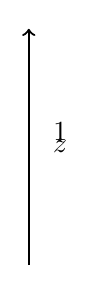
\begin{tikzpicture}[scale=2]
  % Define a variable
  \def\myScalar{1.5} % This is the scalar you want to multiply

  % Draw the arrow
  \draw[->, thick] (0,0) -- (0,\myScalar);
  
  % Label the arrow
  \node at (0.2, \myScalar/2) {$z$};
  \node at (0.2, \myScalar/2 + 0.1) {1}; % Adjust the position of the label if needed
\end{tikzpicture}
\end{document}